\setcounter{section}{-1}
\section{Introductory exercise}
In the introductory lab session, we are taking a look at some basic features of MPI. 

We start out very simple with a hello world program on two nodes. 

\subsection*{Hello World}
\lstinputlisting[language=c]{input/code/00/helloworld1.c}
This program can be compiled with the following command:\\

\begin{verbatim}
mpicc -o helloworld1.out helloworld1.c
\end{verbatim}
And run with:
\begin{verbatim}
srun -n 2 -c 4 --mem-per-cpu=1GB  ./helloworld1.out
\end{verbatim}
We get the following output:
\begin{verbatim}
Node 0 of 2 says: Hello world!
Node 1 of 2 says: Hello world!
\end{verbatim}

From now on I'll skip the compilation and only mention on how many nodes the program is run and what the output is / interpretation of the output.

\subsection{Ping Pong}
I used the template to check how long \texttt{MPI\_Send} and \texttt{MPI\_Recv} take. The code can be found in the appendix for this section. \\

I've modified the printing a bit to make it easier to gather the information. 
Then I piped the program output into a textfile for further processing in python. I ran it first on one and then on two nodes as specified in the assignment sheet. Opposed to the averaging over 5 send / receive pairs, I've done 1000 pairs. Furthmore I reran the whole programm 5 times to gather more data. 
All this data is shown in the following graph: 
% add figure
\begin{figure}[H]
    \centering
    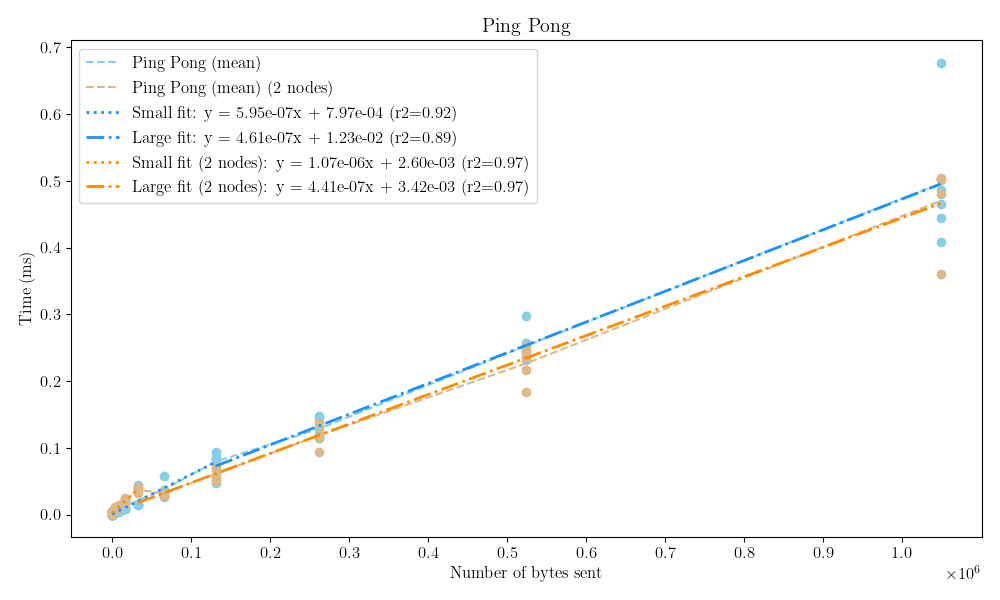
\includegraphics[width=\textwidth]{../fig/lab0/pingPong.png}
    \caption{Ping Pong: Number of bytes sent vs. average time taken from 1000 pairs of send / receive. 5 runs shown for each size as scatter plot. Mean of these 5 runs shown as line. Blue small fit includes all data points up to 131072 bytes, blue large from there. Red small fit includes all data points up to 32768 bytes, red large from there.}
    \label{fig:pingpong}
\end{figure}
As can be seen in the data and the fits, there are outliers especially for the larger data sizes. \\
For our runs we get the following fits and $R^2$ values:
\begin{table}[h!]
    \centering
    \begin{tabular}{|l|l|l|l|}
        \hline
        \textbf{Run Type}   & \textbf{Data Size} & \textbf{Fit Equation}                                      & \textbf{$R^2$ Value} \\ \hline
        \textbf{Single Node} & Small (<=131072)             & $5.95 \times 10^{-7} \cdot x + 7.97 \times 10^{-4}$        & 0.92              \\ \hline
        \textbf{Single Node} & Large (>= 131072)& $4.61 \times 10^{-7} \cdot x + 1.23 \times 10^{-2}$        & 0.89              \\ \hline
        \textbf{Two Node}    & Small (<=32768)& $1.07 \times 10^{-6} \cdot x + 2.60 \times 10^{-3}$        & 0.97              \\ \hline
        \textbf{Two Node}    & Large (>=32768)   & $4.41 \times 10^{-7} \cdot x + 3.42 \times 10^{-3}$        & 0.97              \\ \hline
    \end{tabular}
    \caption{Fit Equations and $R^2$ Values for Single Node and Two Node Runs}
\end{table}

\Shining{Note:} Each run was performed 5 times (for 1 and 2 nodes) to get a fit on the data and calculate a $R^2$ value. 

\subsubsection*{\Shining{Extra: Ping Pong with MPI\_SendRecv}}
We do the same analysis for the changed program utilizing \texttt{MPI\_SendRecv}. The code can be found in the appendix for this section. \\
We get the following graph from the measurements which were performed in the same way as for the previous program:
% add figure
\begin{figure}[H]
    \centering
    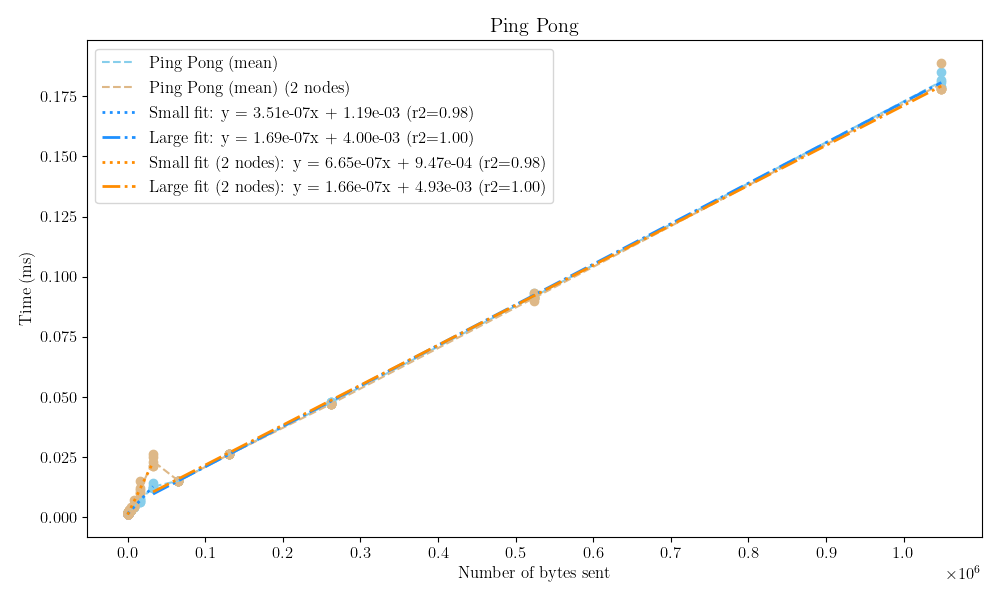
\includegraphics[width=\textwidth]{../fig/lab0/pingPongSR.png}
    \caption{Ping Pong with MPI\_SendRecv: Number of bytes sent vs. average time taken from 1000 pairs of send / receive. 5 runs shown for each size as scatter plot. Mean of these 5 runs shown as line. Blue small fit includes all data points up to 32768 bytes, blue large from there. Red small fit includes all data points up to 32768 bytes, red large from there.}
    \label{fig:pingpongSendRecv}
\end{figure}

We get the following fits and $R^2$ values for the runs:
\begin{table}[h!]
    \centering
    \begin{tabular}{|l|l|l|l|}
        \hline
        \textbf{Run Type}   & \textbf{Data Size} & \textbf{Fit Equation}                                      & \textbf{$R^2$ Value} \\ \hline
        \textbf{Single Node} & Small (<=32768)  & $3.51 \times 10^{-7} \cdot x + 1.19 \times 10^{-3}$        & 0.98              \\ \hline
        \textbf{Single Node} & Large (>=32768)  & $1.69 \times 10^{-7} \cdot x + 4.00 \times 10^{-3}$        & 1.00              \\ \hline
        \textbf{Two Node}    & Small (<=32768)  & $6.65 \times 10^{-7} \cdot x + 9.47 \times 10^{-4}$        & 0.98              \\ \hline
        \textbf{Two Node}    & Large (>=32768)  & $1.66 \times 10^{-7} \cdot x + 4.93 \times 10^{-3}$        & 1.00              \\ \hline
    \end{tabular}
    \caption{Fit Equations and $R^2$ Values for Single Node and Two Node Runs}
\end{table}


\subsection{MM-product}
After an introduction of the matrix-matrix multiplication code in the next section, the measured speedups are discussed in the subsequent section.
\subsubsection*{Explanation of the code}
For this excercise I've used the template provided in the assignment sheet as a base to develop my parallel implementation for a matrix-matrix multiplication. The code can be found in the appendix for this section. \\

The porgam can be run either in sequential (default) or parallel mode (parallel as a command line argument). For the sequential version, the code is practically unchanged and just refactored into a function for timing purposes. The parallel version is more complex and works as explained bellow: \\
First, rank 0 computes a sequential reference solution. Then rank 0 distributes the matrices in the following way in \texttt{splitwork}: 
\begin{itemize}
    \item Matrix A is split row-wise by dividing the number of rows by the number of nodes.
    \item The first worker (=rank 1) gets the most rows starting from row 0: \\$\texttt{total\_rows} - (\texttt{nr\_workers}-1) \cdot \textit{floor}(\frac{\texttt{total\_rows}}{\texttt{nr\_workers}})$.
    \item All other workers and the master (= rank 0) get the same number of rows: $\textit{floor}(\frac{\texttt{total\_rows}}{\texttt{nr\_workers}})$.
    \item The master copies the corresponding rows of matrix A and the whole transposed matrix B\textcolor{cyan}{\textbf{*}} into a buffer (for details on \texttt{MM\_input} buffer see bellow) for each worker and sends them off using \texttt{MPI\_ISend}.
    \item The workers receive the data using \texttt{MPI\_Recv} and then compute their part of the matrix product and send only the rows of the result matrix back to the master using \texttt{MPI\_Send}.
    \item In the meanwhile the master computes its part of the matrix product.
    \item Using \texttt{MPI\_Waitall} the master waits for all data to be sent to the workers and only afterwards calls \texttt{MPI\_Recv} to gather the results from the workers.
    \item Finally all results are gathered by the master in the result matrix.
\end{itemize}
Assume we have a 5x5 matrix $A$ and 2 workers (rank 1 and rank 2) and master (rank 0). The partitioning is done row-wise as follows:
\begin{tcolorbox}[examplebox, title=Partitioning Example]

\[
A =
\begin{pmatrix}
    a_{11} & a_{12} & a_{13} & a_{14} & a_{15} \\
    a_{21} & a_{22} & a_{23} & a_{24} & a_{25} \\
    a_{31} & a_{32} & a_{33} & a_{34} & a_{35} \\
    a_{41} & a_{42} & a_{43} & a_{44} & a_{45} \\
    a_{51} & a_{52} & a_{53} & a_{54} & a_{55} \\
\end{pmatrix} \rightarrow
\begin{pmatrix}
    \text{Worker 1} \\
    \text{Worker 1} \\
    \text{Worker 1} \\
    \text{Master} \\
    \text{Master} \\
\end{pmatrix}
\]

\begin{itemize}
    \item \textbf{Rank 0 (Master)}: Rows 4 and 5 (last two rows)
    \item \textbf{Rank 1 (Worker 1)}: Rows 1 to 3 (first three rows) - Worker 1 always gets the most rows
\end{itemize}

This partitioning can be visually represented as:

\[
\text{Master (rank 0):}
\begin{pmatrix}
    a_{41} & a_{42} & a_{43} & a_{44} & a_{45} \\
    a_{51} & a_{52} & a_{53} & a_{54} & a_{55} \\
\end{pmatrix}
\]

\[
\text{Worker 1 (rank 1):}
\begin{pmatrix}
    a_{11} & a_{12} & a_{13} & a_{14} & a_{15} \\
    a_{21} & a_{22} & a_{23} & a_{24} & a_{25} \\
    a_{31} & a_{32} & a_{33} & a_{34} & a_{35} \\
\end{pmatrix}
\]

\end{tcolorbox}
Each worker computes its part of the matrix product, and the master gathers the results at the end and compiles them into the final matrix.

The \texttt{MM\_input} buffer is used to store the rows of matrix A and the whole matrix B for each worker. It is implemented using a simple struct:
\begin{lstlisting}[language=c]
typedef struct MM_input {
    size_t rows;
    double *a;
    double *b;
} MM_input;
\end{lstlisting}

\Shining{*[Optimization] Note on transposed matrix B:} It is usually beneficial from a cache perspective to index arrays sequentially or in a row-major order. However, in the matrix-matrix multiplication, we access the elements of matrix B in a column-wise order. This leads to cache misses and is not optimal. To mitigate this, we can transpose matrix B and then access it in a row-wise order. This is done in the code by the master before sending the data to the workers.

\subsubsection*{Discussion of the speedups}
The code was run on Delft's cluster with 1, 2, 4, 8, 16, 24, 32, 48, and 64 nodes. For the experiments the matrix size of $A$ and $B$ was set to $2000\times2000$. 
This means that the program has to evaluate $2000$ multiplications and $1999$ additions for each element of the resulting matrix $C$. In total this results in $\approx 2000^3 = 8 \times 10^9$ operations.\\
The command looked similar to the following for the different node counts:
\begin{verbatim}
srun -n 48 --mem-per-cpu=4GB --time=00:02:00 ./MM.out parallel
\end{verbatim}
For this experiment, the execution time was measured and the speedup was calculated. The results are shown in \autoref{tab:execution_time} and \autoref{fig:speedup}.

\begin{table}[h!]
    \centering
    \begin{tabular}{|c|c|c|}
        \hline
        \textbf{CPU Count} & \textbf{Execution Time / s} & \textbf{Approx. Speedup} \\ 
        \hline
        1   & 47.11  & 1.0 \\ 
        2   & 10.26  & 4.6 \\ 
        4   & 10.30  & 4.6 \\ 
        8   &  5.20  & 9.1 \\ 
        16  &  2.97  & 15.9 \\ 
        24  &  2.54  & 18.5 \\ 
        32  &  2.29  & 20.6 \\ 
        48  &  2.98  & 15.8 \\ 
        64  &  1.72  & 27.4 \\ 
        \hline
    \end{tabular}
    \caption{Execution Time vs CPU Count}
    \label{tab:execution_time}
\end{table}

\begin{figure}[H]
    \centering
    \includegraphics[width=0.8\textwidth]{../fig/lab0/MM\_plot.png}
    \caption{Speedup vs CPU Count\\
    Black $\times$ marks the average of the rerun for $n=48$.}
    \label{fig:speedup}
\end{figure}

\Shining{Note:} The speedup is calculated as $S = \frac{T_1}{T_p}$, where $T_1$ is the execution time on 1 node and $T_p$ is the execution time on $p$ nodes.\\

\textbf{Discussion:}\\
As one can cleary discern from the data in \autoref{tab:execution_time} and \autoref{fig:speedup}, the speedup increases with the number of nodes (with the exception of $n=48$). This is expected as the more nodes we have, the more work can be done in parallel. However, the speedup is not linear. This is due to the overhead of communication between the nodes. The more nodes we have, the more communication is needed, and this overhead increases. This is especially visible in the data for $n=48$. Here the speedup is lower than for $n=32$. For this run the communication didn't went as smooth as for the other runs. This can potentially be attributed to the fact that one (or more) of the nodes or the network was under heavy load during this task. \\

\Shining{[Further investigation]} After observing this slower speed for the $n=48$, I reran the tests multiple times and got a runtime of around $1.9 s$ which was to be expected initially. Therefore, this one run is an odd one out, most likely due to the reasons mentioned above! I've also added the averaged data of the reruns as a datapoint in \autoref{fig:speedup}.\\
Another interesting fact can be seen when comparing the time taken for $n=1$ and $n=2$. They don't at all scale with the expected factor of 2. This is could be due to the fact, that the resource management system prefers runs with multiple nodes instead of a single node (= sequential). \\

Additional notes: The flag \texttt{--mem-per-cpu=<\#>GB} was set depending on the number of nodes used. For 1-24 nodes 8GB was used, for 32-48 nodes 4GB, and for 64 nodes 3GB. This had to be done to comply with QOS policy on the cluster. 

% \TODO{Data locality?}








